\documentclass[11pt,a4paper]{article}
\usepackage[margin=21mm]{geometry}
\usepackage{amsmath,amssymb,booktabs,array}
\usepackage{tikz}
\usepackage[T1]{fontenc}
\usepackage{lmodern}
\usepackage{xcolor}
\usepackage{hyperref}
\hypersetup{colorlinks=true,linkcolor=blue,urlcolor=blue}
\setlength{\parindent}{0pt}
\setlength{\parskip}{6pt}
\newcommand{\DD}{V_{\mathrm{DD}}}
\newcommand{\GND}{\mathrm{GND}}
\newcommand{\N}[1]{\mathrm{N}(#1)}
\newcommand{\Pmos}[1]{\mathrm{P}(#1)}
\newcommand{\NM}[4]{%
  \coordinate (#1t) at (#2,{#3+.5});\coordinate (#1b) at (#2,{#3-.5});
  \draw (#1t)--(#2,{#3+.28})--({#2+.12},{#3+.28})--({#2+.12},{#3-.28})--(#2,{#3-.28})--(#1b);
  \draw ({#2-.14},{#3-.2})--({#2-.14},{#3+.2});
  \draw ({#2-.55},#3)--({#2-.14},#3);
  \node[anchor=east] at ({#2-.62},#3) {$#4$};}
\newcommand{\PM}[4]{%
  \coordinate (#1t) at (#2,{#3+.5});\coordinate (#1b) at (#2,{#3-.5});
  \draw (#1t)--(#2,{#3+.28})--({#2+.12},{#3+.28})--({#2+.12},{#3-.28})--(#2,{#3-.28})--(#1b);
  \draw ({#2-.14},{#3-.2})--({#2-.14},{#3+.2});
  \draw ({#2-.55},#3)--({#2-.35},#3);
  \draw ({#2-.295},#3) circle[radius=.055];
  \draw ({#2-.24},#3)--({#2-.14},#3);
  \node[anchor=east] at ({#2-.62},#3) {$#4$};}
\newcommand{\groundat}[2]{\draw (#1,#2)--(#1,{#2-.13});
  \draw ({#1-.28},{#2-.13})--({#1+.28},{#2-.13});
  \draw ({#1-.18},{#2-.22})--({#1+.18},{#2-.22});
  \draw ({#1-.08},{#2-.31})--({#1+.08},{#2-.31});}
\newcommand{\AOIcircuit}[5]{%
\begin{tikzpicture}[line width=.8pt,x=.9cm,y=.9cm]
  \PM{P1}{.8}{6.1}{#1}\PM{P2}{3.8}{6.55}{#2}\PM{P3}{3.8}{5.45}{#3}
  \PM{P4}{.8}{3.95}{#4}\PM{P5}{3.8}{3.95}{#5}
  \draw (.8,7.2)--(3.8,7.2);\draw (2.3,7.2)--(2.3,7.5) node[above] {$\DD$};
  \draw (P1t)--(.8,7.2);\draw (P2t)--(3.8,7.2);\draw (P2b)--(P3t);
  \draw (P1b)--(.8,4.8)--(3.8,4.8)--(P3b);
  \draw (P4t)--(.8,4.8);\draw (P5t)--(3.8,4.8);
  \draw (P4b)--(.8,3.2)--(3.8,3.2)--(P5b);
  \draw (3.8,3.2)--(5.1,3.2) node[right] {$f$};
  \fill (3.8,3.2) circle[radius=.05];
  \NM{N1}{.8}{2.4}{#1}\NM{N2}{0}{1}{#2}\NM{N3}{1.7}{1}{#3}
  \NM{N4}{3.8}{2.4}{#4}\NM{N5}{3.8}{1}{#5}
  \draw (N1t)--(.8,3.2);\draw (N4t)--(3.8,3.2);\draw (N4b)--(N5t);
  \draw (N1b)--(.8,1.7);\draw (0,1.7)--(1.7,1.7);
  \draw (N2t)--(0,1.7);\draw (N3t)--(1.7,1.7);
  \draw (N2b)--(0,.3)--(3.8,.3)--(N5b);\draw (N3b)--(1.7,.3);
  \groundat{2.3}{.3}
  \node[anchor=west,font=\small,text=gray] at (5.1,5.5) {PUN};
  \node[anchor=west,font=\small,text=gray] at (5.1,1.7) {PDN};
\end{tikzpicture}}

\begin{document}

\begin{center}{\Large\bfseries 2013 Homework 2}\par Slew, clock-tree delay, mobility and noise margins\end{center}
The original printed prompt is preserved at \texttt{../assignments/homework2.pdf}.
Both handwritten answer photographs by student 100501015 were reviewed before
derivation. They give the correct main conclusions; the qualifications and
unit checks below make their assumptions explicit.

\section*{1. Faster rising input gives faster output fall}
For the given inverter and fixed load,
\[
 C_L\frac{dV_{out}}{dt}=I_p-I_n.
\]
The NMOS begins conducting when $V_{in}>V_{tn}$; the PMOS remains conducting
while $V_{in}<V_{DD}-|V_{tp}|$. With input waveform a, the input reaches strong
NMOS overdrive sooner and turns the competing PMOS off sooner. Therefore the
net load-discharge current is larger during the transition, and the output
falls faster. Waveform b spends more time with a weaker NMOS and simultaneous
PMOS pull-up. This explains the stated fall-time ordering.

\begin{center}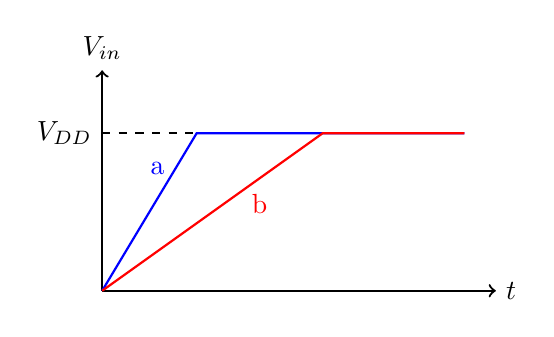
\begin{tikzpicture}[line width=.8pt]
\draw[->] (0,0)--(5,0) node[right] {$t$};\draw[->] (0,0)--(0,2.8) node[above] {$V_{in}$};
\draw[dashed] (0,2)--(4.6,2);\node[left] at (0,2) {$V_{DD}$};
\draw[blue,thick] (0,0)--(1.2,2)--(4.6,2);\node[blue] at (.7,1.55) {a};
\draw[red,thick] (0,0)--(2.8,2)--(4.6,2);\node[red] at (2,1.1) {b};
\end{tikzpicture}\end{center}
The reference uses the halfway point as an informal transition marker.
Actual device turn-on/off voltages depend on thresholds; neither transistor
universally switches off exactly at $V_{DD}/2$. The statement concerns the
specified inverter experiment, not an unconditional bound for every circuit.

\section*{2. Critical path of the printed clock tree}
The output-C buffer is labeled $2\tau_g$, while the A, B and D buffers have
delay $\tau_g$. Use the prompt's $r=0.05\,\Omega/\mu$m and
$c=30\times10^{-18}$ F/$\mu$m. For an isolated length $l$ in $\mu$m,
\[
 \tau_w=\tfrac12rcl^2=0.75\times10^{-18}l^2\ \mathrm{s}.
\]
The printed neglect criterion is $\tau_w\le4\tau_g=0.8$ ns, not
$\tau_g/4$. A 200 $\mu$m segment gives 0.030000 ps; a 250 $\mu$m segment
gives 0.046875 ps. Even the following whole-path estimates are negligible:
\begin{center}\begin{tabular}{lrrr}\toprule
Path&Wire length ($\mu$m)&$\tfrac12rcl^2$ (ps)&Gate delay (ns)\\\midrule
A to B&650&0.316875&0.4\\A to C&400&0.120000&0.6\\A to D&650&0.316875&0.4\\\bottomrule
\end{tabular}\end{center}
\[\boxed{\text{Critical path: A to C; delay }3\tau_g=0.6\text{ ns}.}\]
The handwritten answer obtains the same result and properly uses 4$\tau_g$.
A branched tree's exact Elmore delay includes downstream branch loading and
unspecified gate capacitances; the isolated-wire formula is the stated course
approximation. The problem explicitly permits neglecting these very small
wire terms, so they are not added as an exact physical tree-delay prediction.

\newpage\section*{3. Mobility ratio at the switching point}
At $V_{in}=V_{out}=V_{DD}/2$, both conducting devices are saturated in the
ideal long-channel model. With common $C_{ox}$, equal currents give
\[
 \mu_n\cdot2\,(V_{DD}/2-V_{tn})^2
 =\mu_p\cdot4\,(V_{DD}/2-|V_{tp}|)^2.
\]
Hence the general relation is
\[
 \boxed{\frac{\mu_n}{\mu_p}
 =2\left(\frac{V_{DD}/2-|V_{tp}|}{V_{DD}/2-V_{tn}}\right)^2.}
\]
Under the usual implicit matched-threshold assumption $V_{tn}=|V_{tp}|$,
\[\boxed{\mu_n/\mu_p=2,}\]
as in the supplied answer. Unequal threshold magnitudes or oxide capacitances
would prevent the two midpoint voltages alone from determining mobility uniquely.

\section*{4. Design for $NM_H>NM_L$}
\[
 NM_H=V_{OH}-V_{IH},\qquad NM_L=V_{IL}-V_{OL}.
\]
With matched threshold magnitudes and nearly ideal rail outputs, make the NMOS
pull-down stronger than the PMOS pull-up:
\[
 \boxed{\beta_n>\beta_p,\quad
 \mu_n(W_n/L_n)>\mu_p(W_p/L_p).}
\]
Increasing $W_n/L_n$ or decreasing $W_p/L_p$ shifts the voltage-transfer curve
left. The inverter accepts a lower input voltage as high, reducing $V_{IH}$
and increasing $NM_H$; it also reduces $V_{IL}$ and thus $NM_L$. If
$\mu_n=2\mu_p$ and lengths are equal, require $W_p<2W_n$ for this strength
ordering. A stronger PMOS would shift the characteristic in the opposite direction.

\begin{center}\begin{tabular}{rrr}\toprule
$\beta_n/\beta_p$&$NM_L$ (V)&$NM_H$ (V)\\\midrule
0.25&0.984360&0.603557\\
0.5&0.889328&0.688420\\
1&0.787500&0.787500\\
2&0.688420&0.889328\\
4&0.603557&0.984360\\
\bottomrule\end{tabular}\end{center}
The table is an illustrative square-law check at $V_{DD}=1.8$ V and equal
threshold magnitudes 0.45 V. It solves the $dV_{out}/dV_{in}=-1$ boundaries;
these are not values specified by the assignment or measured with CIC018.

\textbf{Reference decisions.} Retain the supplied faster-slew explanation,
A-to-C critical path, mobility ratio 2 and $\beta_p<\beta_n$ sizing.
Use threshold-dependent current balance instead of treating resistance matching
as a universal transistor identity. Distinguish the transfer curve's switching
point from the formal noise-margin slope boundaries.

\textbf{Verification.} \texttt{python verify.py} checks three clock paths and
five ideal noise-margin examples. Results are in \texttt{clock\_tree.csv},
\texttt{noise\_margin.csv} and \texttt{verification.json}. These four questions
are analytical; the prompt does not request a SPICE experiment.

\end{document}
